%!TEX spellcheck
%!TEX root = ../bachelor_paper.tex
\documentclass[../bachelor_paper.tex]{subfiles}
\graphicspath{{\subfix{images/}}}
\begin{document}

\chapter{Results}
    \label{ch:res}

We were able to successfully generate performance profiles for the workloads described in Section \ref{sec:bench/sum}. The most noteworthy results are presented and analyzed in the section bellow. Graphs for the workloads we have not presented specifically in this chapter can be found in Appendix \ref{app:graphs}.

\section{Instruction distribution}
The workloads vary highly in instruction distribution, however for most of them arithmetic instructions make up the majority of instructions in many workloads (see Figure \ref{fig:res/overall/inst}). Exception to these rules are \texttt{embench edn}, \texttt{embench matmult int}, \texttt{embench nsichneu}, and \texttt{riscv vvadd} with load instructions as the dominant type; \texttt{embench statemate} with store instructions as the dominant type; as well as \texttt{riscv median} with branching instructions as the dominant type. As can be seen in Figure \ref{fig:res/overall/inst}, the difference between the most favored category and the runner up appears to be rather large on average. Indeed, the mean difference between the first two categories over all 39 workloads is 32.11\% points, where only 7 workloads have a disparity of less than 10\% points, with 25 having a disparity of over 20\% points and 17 having a disparity greater than the mean. This indicates that each workload strongly prefers one type of instruction with arithmetic instructions being the clear overall favorite. 

Moreover, we can see that almost no workload we tested uses FPU instructions, with \texttt{embench minver} being the only significant contender with a share of 13.8\%. Only \texttt{mibench-automotive susan} and \texttt{mibench-telecomm FFT} even register with a share of 0.21\% and 0.01\% respectively.

%% Overall
\begin{figure}
    \centering
    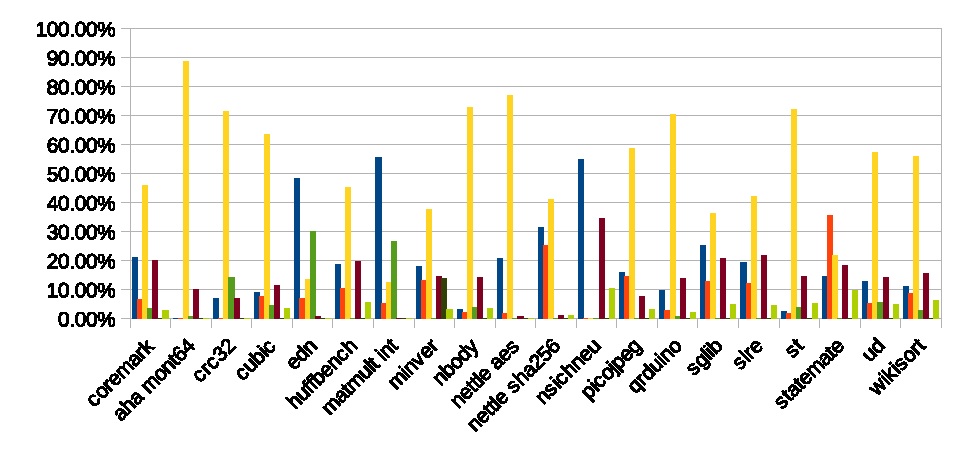
\includegraphics[width=\textwidth]{img/graph/overall_inst_dist}
    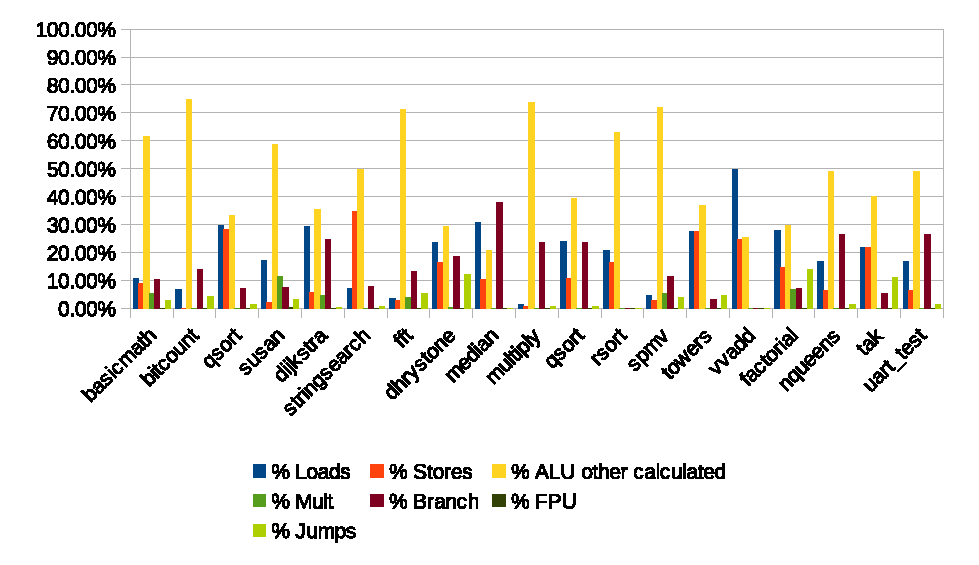
\includegraphics[width=\textwidth]{img/graph/overall_inst_dist2}
    \caption{Overall instruction distribution of all tested benchmarking workloads}
    \label{fig:res/overall/inst}
\end{figure}

\section{Control flow behavior}
    \label{sec:res/control}
As seen in Figure \ref{fig:res/overall/branch_tk}, a vast majority of benchmarks take more than 50\% of branches. Given RI5CY's \emph{branch-not-taken}-strategy, this leads to a high percentage of failed branch predictions. Only 10 workloads take less than 50\% of branches.

Not all tested workloads employ \acp{HWL}. In workloads which do use \acp{HWL}, usage modes vary a lot depending on the implemented algorithm. An extreme example of \ac{HWL} use is \texttt{embench crc32} with a mean distance between initializations of $39 \cdot 10^6$ as well as a mean iteration count of $2.7 \cdot 10^6$ as can be seen in Figure \ref{fig:res/overall/hwl} which is by far the highest number in both distance between initializations and iteration count. We suspect there to be a correlation between these two metrics in extreme cases like this, as no further \ac{HWL} initialization happens during the run of the loop (thus inflating mean distance between \ac{HWL} initializations). More work would be needed to determine whether this correlation is an issue for similarity assessment and, if so, how it could be mitigated.

\begin{figure}
    \centering
    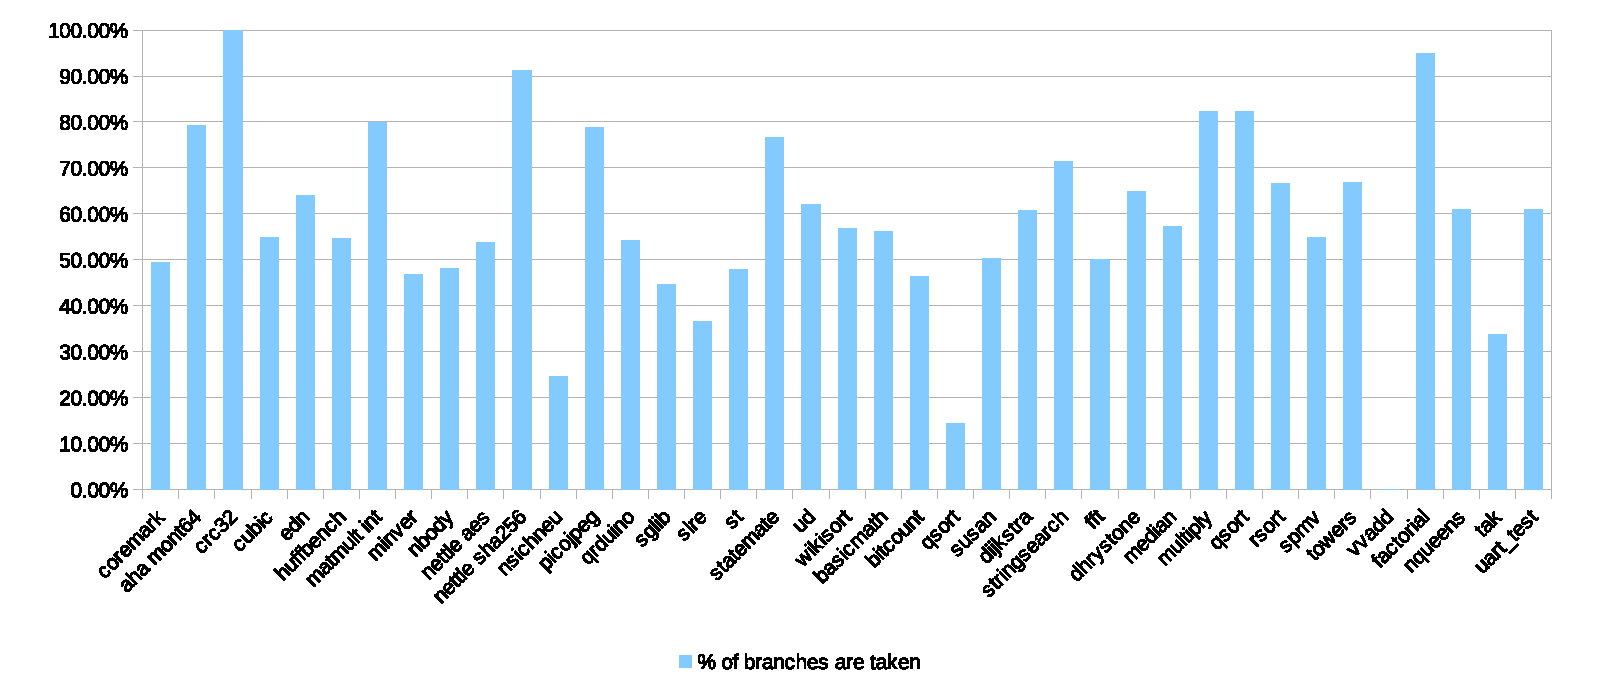
\includegraphics[width=\textwidth]{img/graph/overall_branch_tk.eps}
    \caption{Overall branch taken behavior of all tested benchmarking workloads}
    \label{fig:res/overall/branch_tk}
\end{figure}

\begin{figure}
    \centering
    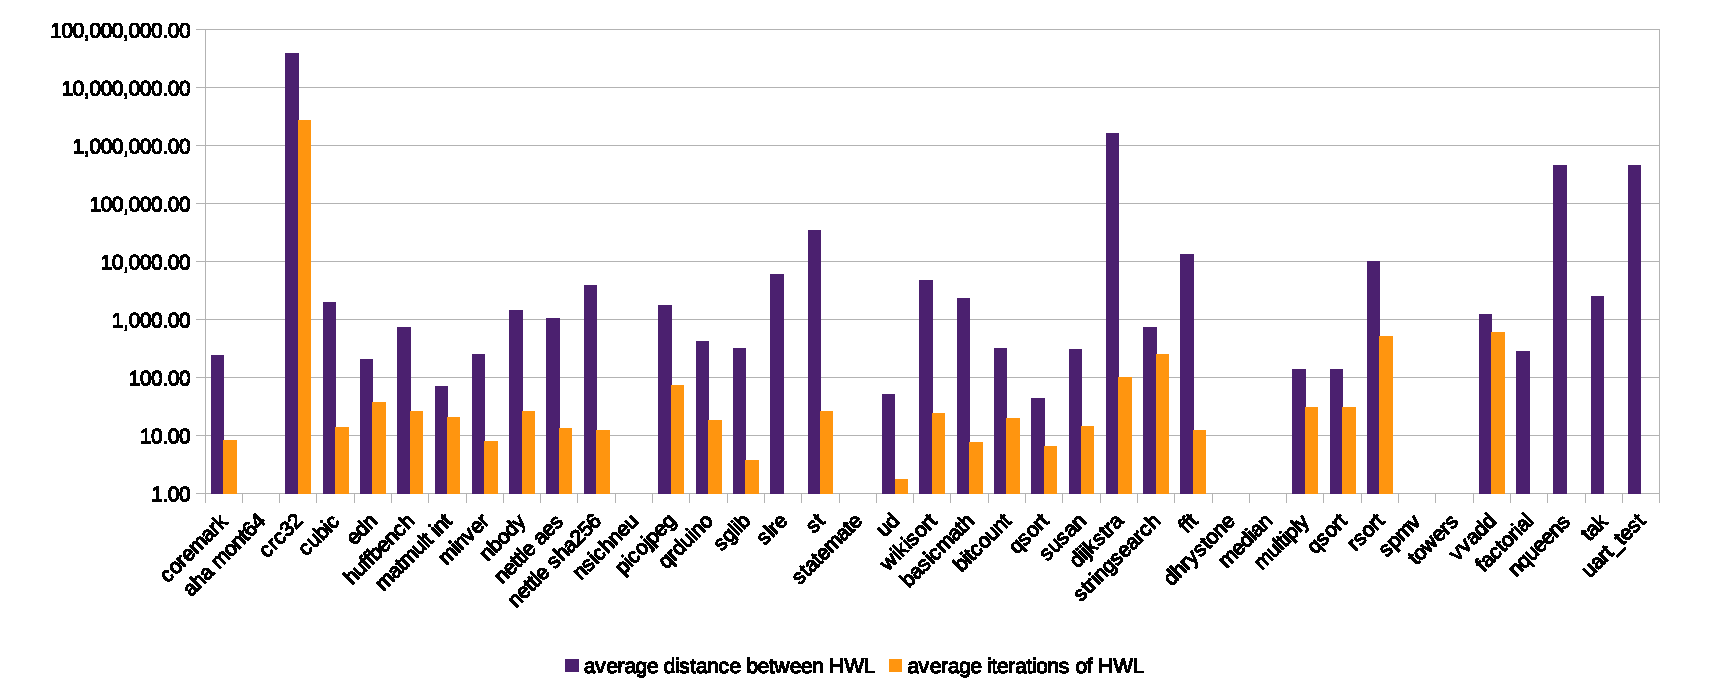
\includegraphics[width=\textwidth]{img/graph/overall_hwl.eps}
    \caption{Overall hardware loop behavior of all tested benchmarking workloads}
    \label{fig:res/overall/hwl}
\end{figure}

\section{Instruction load efficiency}
As described in Section \ref{sec:res/control}, a majority of workloads have a branch taken rate of higher than 50\%. The logical assumption would be a higher load coefficient and thus lower instruction load efficiency in these workloads. We have found the relation to be more complicated however. In fact, all five programs with a load coefficient less than 1 (meaning less instructions loaded from level 2 than executed thus higher instruction load efficiency) have a branch taken percentage well above 50\%, as can be seen in Figure \ref{fig:res/overall/fetch_waste} (we intentionally excluded \texttt{tak} included in the \emph{custom} set here, as it only executes 2555 instructions and is thus too small to draw conclusions from). A high branch taken rate does not necessitate poor instruction load efficiency. A low branch taken rate does not necessitate a high instruction load efficiency either. \texttt{embench nsichneu} has a branch taken rate of $24.6\%$, yet a load coefficient of $1.55$.

We suspect loop length to play a considerable role in determining the instruction load efficiency in regard to the harsh constraint of a 4 instruction prefetch buffer. \texttt{embench nettle aes} and \texttt{embench nettle sha256} have a branch taken rate of 53.68\% and 91.22\% but a fetch coefficient of 0.91 and 0.71 respectively. \texttt{embench nbody} is similar to \texttt{embench nettle aes} in all metrics, yet has a significantly higher load coefficient. This suggests that \texttt{embench nettle aes} has a smaller loop body size than \texttt{embench nettle aes} overall and therefor requires less instruction fetches from level 2. Additionally, we suspect instruction alignment to play a large role as well, as adding single instructions at the beginning and end of functions was able to change benchmark performance significantly. Further work would be required to confirm this hypothesis.

\begin{figure}
    \centering
    \includegraphics[width=\textwidth]{img/graph/overall_fetch_waste.eps}
    \caption{Overall load coefficient and cycles wasted per instruction of all tested benchmarking workloads}
    \label{fig:res/overall/fetch_waste}
\end{figure}

\section{Temporal behavior}
Lastly, we have identified three major types of workloads given their temporal behavior. Benchmarks below a certain length have been excluded from this categorization as they did not produce adequate data for analysis. The graphs of those which have been analyzed can be found in Appendix \ref{app:graphs}. We have defined three major groups from the generated data, ranging from completely static to extreme behavioral variation or oscillation.

Group 1 does not change its behavior significantly over the duration of the benchmark. All metrics are unchanged over the course of the entire run. One example for group 1 is Dhrystone as seen in Figure \ref{fig:res/dhrystone}. The \ac{HWL} graph for Dhrystone is missing, as Dhrystone does not utilize \acp{HWL}. Dhrystone exhibits a branch taken rate in the middle- to high range compared to other workloads, as can be seen in Figure \ref{fig:res/overall/branch_tk}, with \ac{ALU} instructions being the prevalent type. What is particularly interesting about Dhrystone is the completely static nature of its metrics. Over the entire benchmark duration of about 2.9 seconds behavior does not change, indicating possibly a short workload that is repeated until an end condition is met. This program loop is very likely a \texttt{while} loop with a non precomputable iteration count, as no \acp{HWL} are used (indicated by the missing \ac{HWL} graph).

% dhrystone   
\begin{figure}
    \begin{subfigure}{\textwidth}
        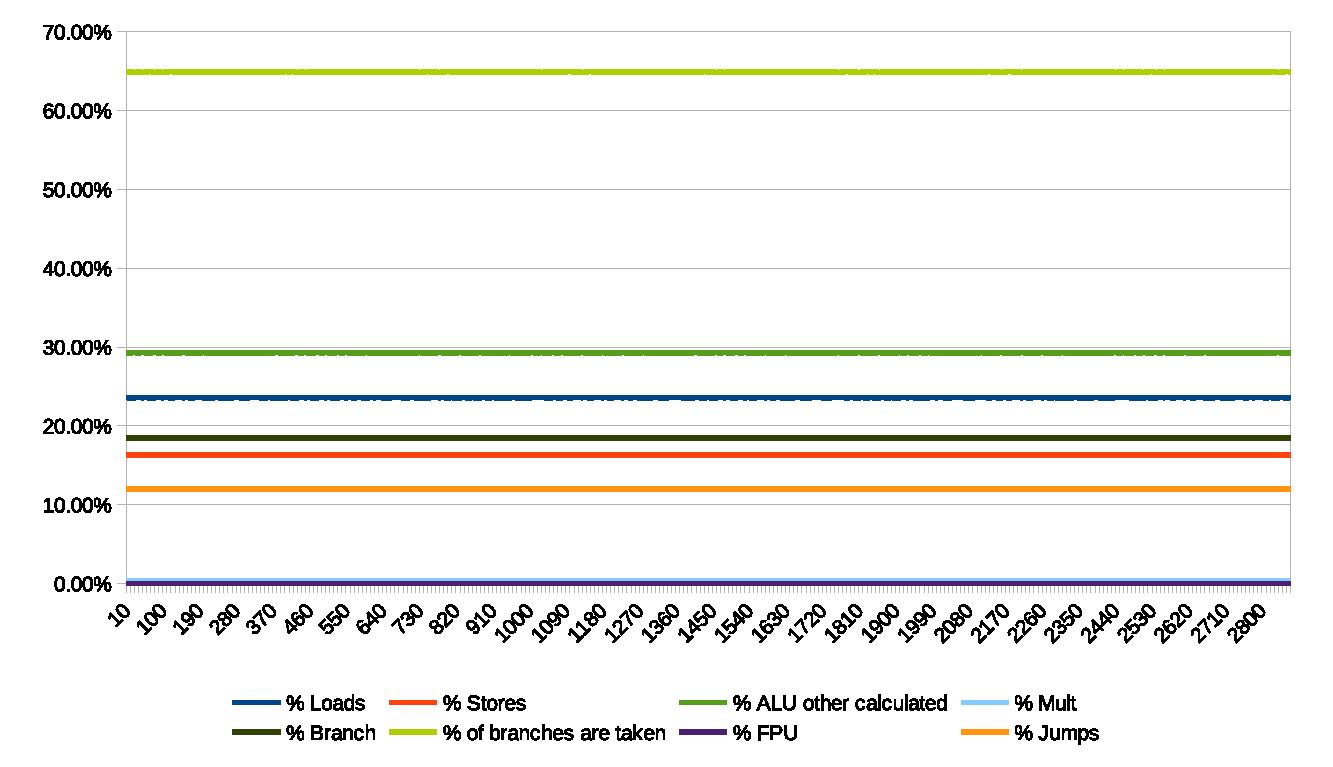
\includegraphics[width=\textwidth]{img/graph/riscv/dhrystone_inst.eps}
        \caption{Instruction behavior over time (ms)}
        \label{fig:res/dhrystone/inst}
    \end{subfigure}
    \begin{subfigure}{\textwidth}
        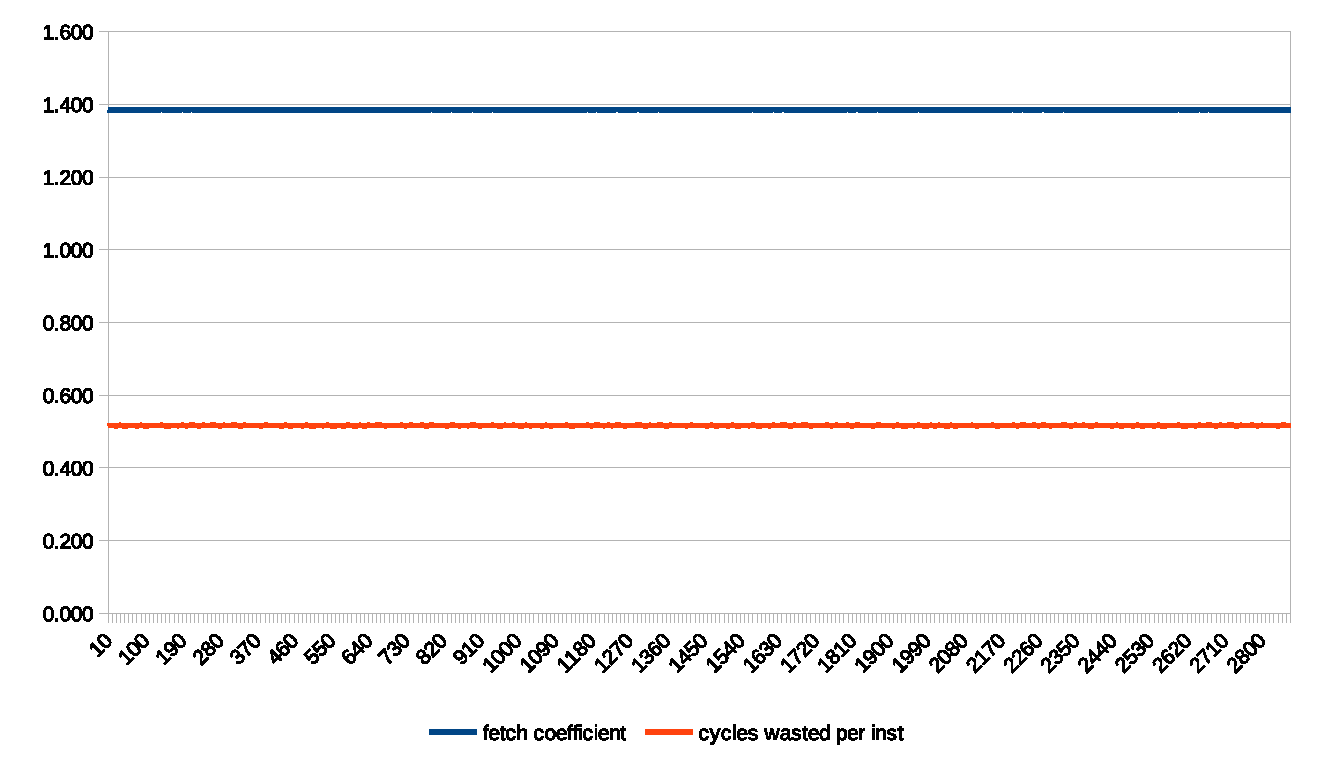
\includegraphics[width=\textwidth]{img/graph/riscv/dhrystone_fetch_waste.eps}
        \caption{Fetch coefficient and cycles wasted per instruction over time (ms)}
        \label{fig:res/dhrystone/fetch_waste}
    \end{subfigure}
    \caption{Performance over time: Dhrystone}
    \label{fig:res/dhrystone}
\end{figure}

Group 2 shows sectional behavioral variation, where sections have relatively stable behavior with stark changes between sections. An example for group 2 is \texttt{mibench-} \texttt{automotive bitcount}, the temporal behavior graphs of which can be seen in Figure \ref{fig:res/bitcount}. The workload displays 7 distinct regions, which hint at different program loops being executed. All regions except the first and last display little to no change in metrics with short initialization phases at the transients. The first 6 sections appear to be implemented using \texttt{while} without precomputable iteration counts not unlike Dhrystone, as no \acp{HWL} are used. Section 7 does seem to use precomputable loops, as the usage of \acp{HWL} is indicated here (see Figure \ref{fig:res/bitcount/hwl}).

% bitcount   
\begin{figure}
    \centering
    \begin{subfigure}{\textwidth}
        \centering
        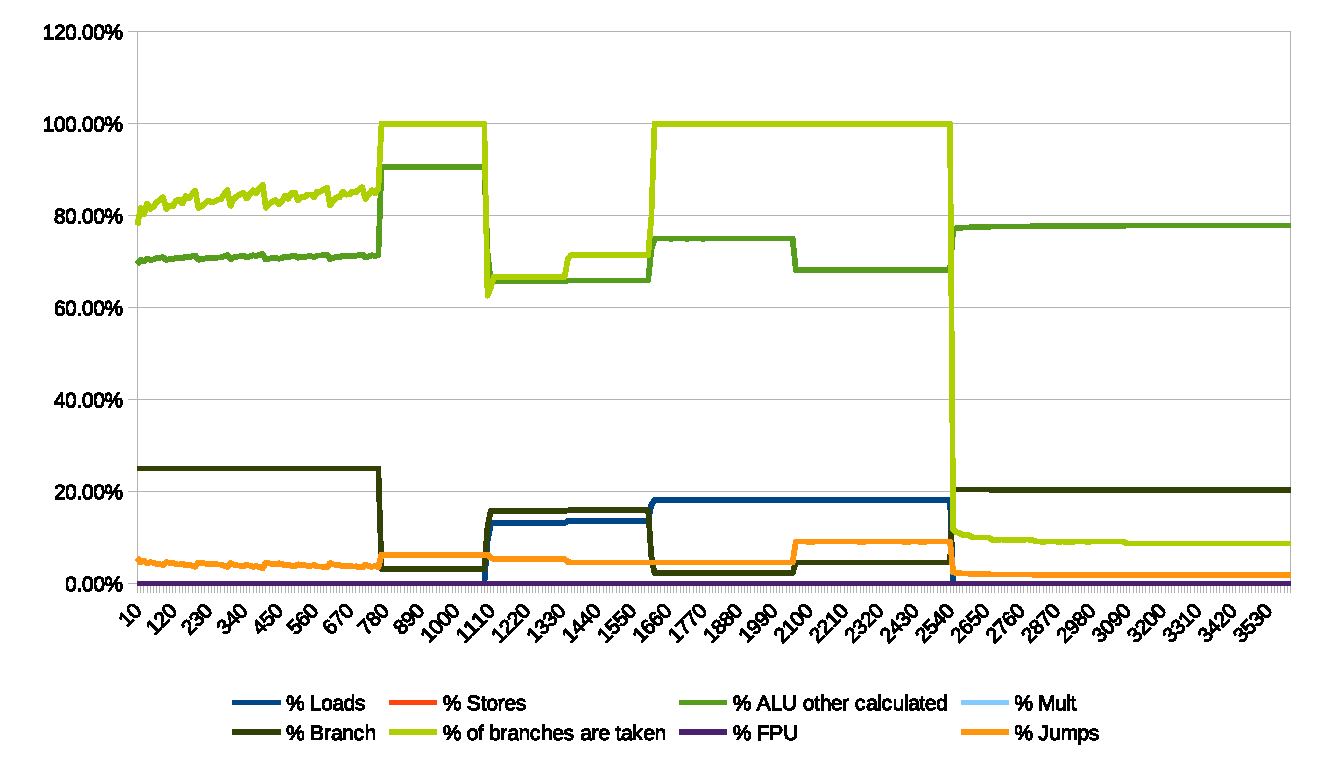
\includegraphics[height=0.26\textheight]{img/graph/mibench/bitcount_inst.eps}
        \caption{Instruction behavior over time (ms)}
        \label{fig:res/bitcount/inst}
    \end{subfigure}
    \begin{subfigure}{\textwidth}
        \centering
        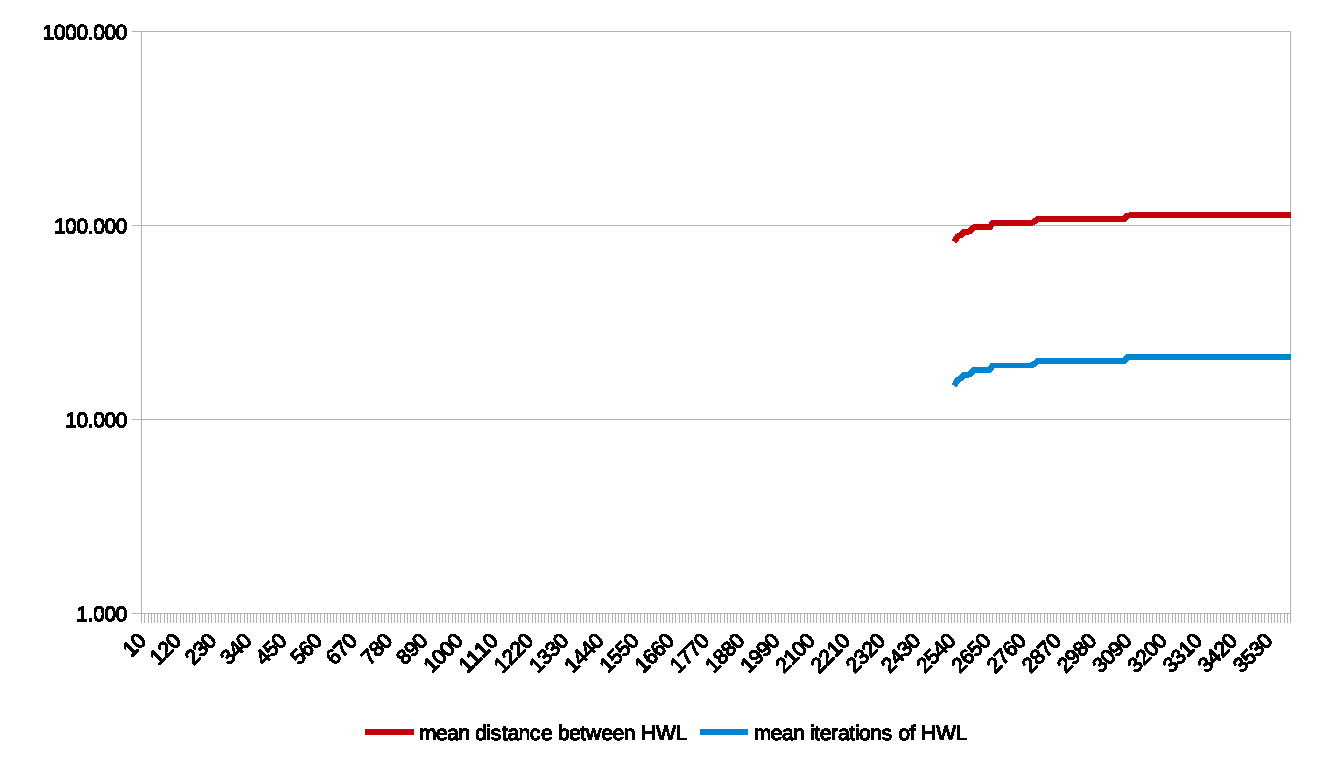
\includegraphics[height=0.26\textheight]{img/graph/mibench/bitcount_hwl.eps}
        \caption{\ac{HWL} behavior over time (ms)}
        \label{fig:res/bitcount/hwl}
    \end{subfigure}
    \begin{subfigure}{\textwidth}
        \centering
        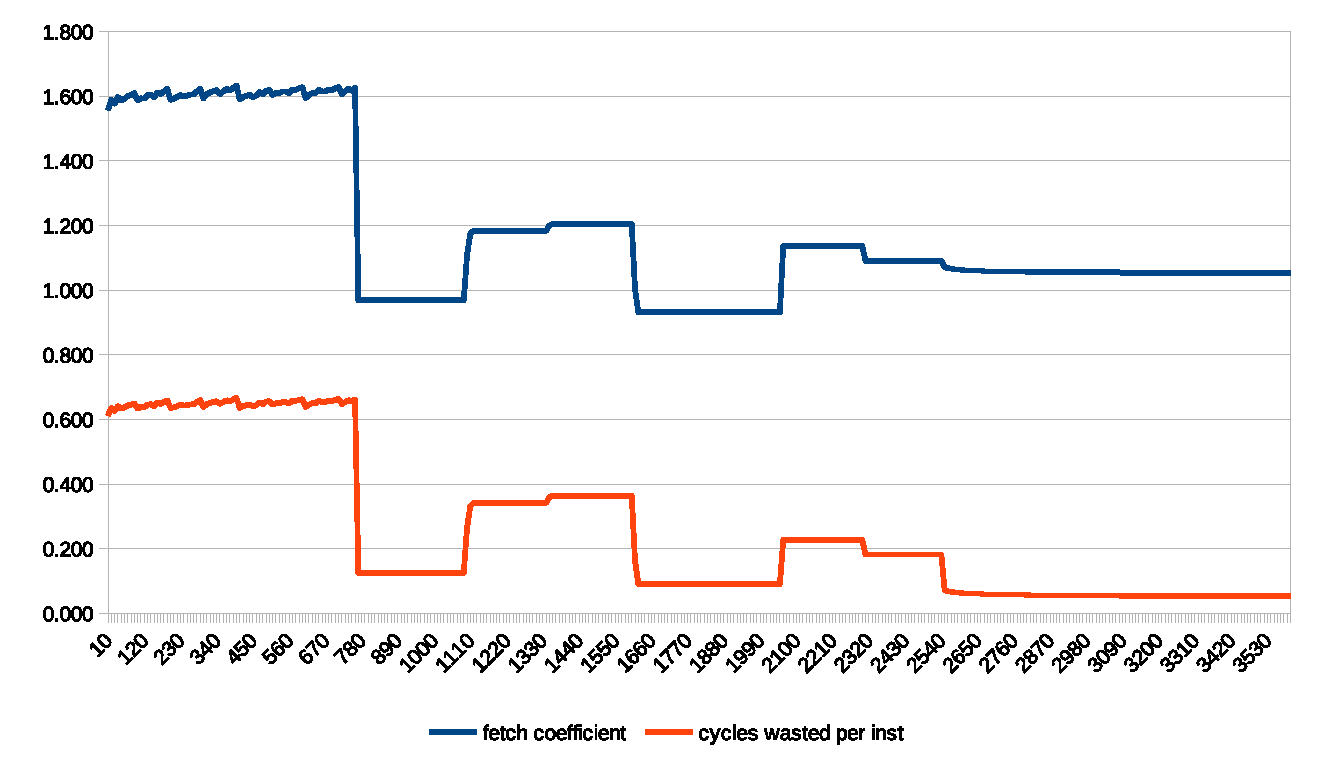
\includegraphics[height=0.26\textheight]{img/graph/mibench/bitcount_fetch_waste.eps}
        \caption{Fetch coefficient and cycles wasted per instruction over time (ms)}
        \label{fig:res/bitcount/fetch_waste}
    \end{subfigure}
    \caption{Performance over time: \texttt{bitcount}}
    \label{fig:res/bitcount}
\end{figure}

Group 3 fluctuates strongly during the entire duration of the benchmark. Examples for group 3 are the synthetic Coremark, as can be seen in Figure \ref{fig:res/coremark}, as well as \texttt{embench sglib-combined}, as seen in Figure \ref{fig:res/sglib}. Both see more or less drastic variation within all metrics measured, with \texttt{embench sglib-combined} displaying behavior reminiscent of oscillation. Coremark seems to exhibit repetition of behavioral patterns, as a zoom into the graph reveals relatively periodic sections, which does match the makeup of Coremark outlined in Section \ref{sec:bench:coremark}. \texttt{embench sglib-combined} also displays strong variation of metrics, however the variation range is much less drastic than with Coremark. The benchmark displays 4 different sections, which are best exemplified by Figure \ref{fig:res/sglib/hwl}. When the initialization distance between \acp{HWL} drops, so does the variation of share of \ac{ALU} instructions. While \texttt{embench sglib-combined} has a relatively stable fetch coefficient around 1.2, Coremark does fluctuate wildly between 1.15 and 1.3.


% Coremark   
\begin{figure}
    \begin{subfigure}{\textwidth}
        \centering
        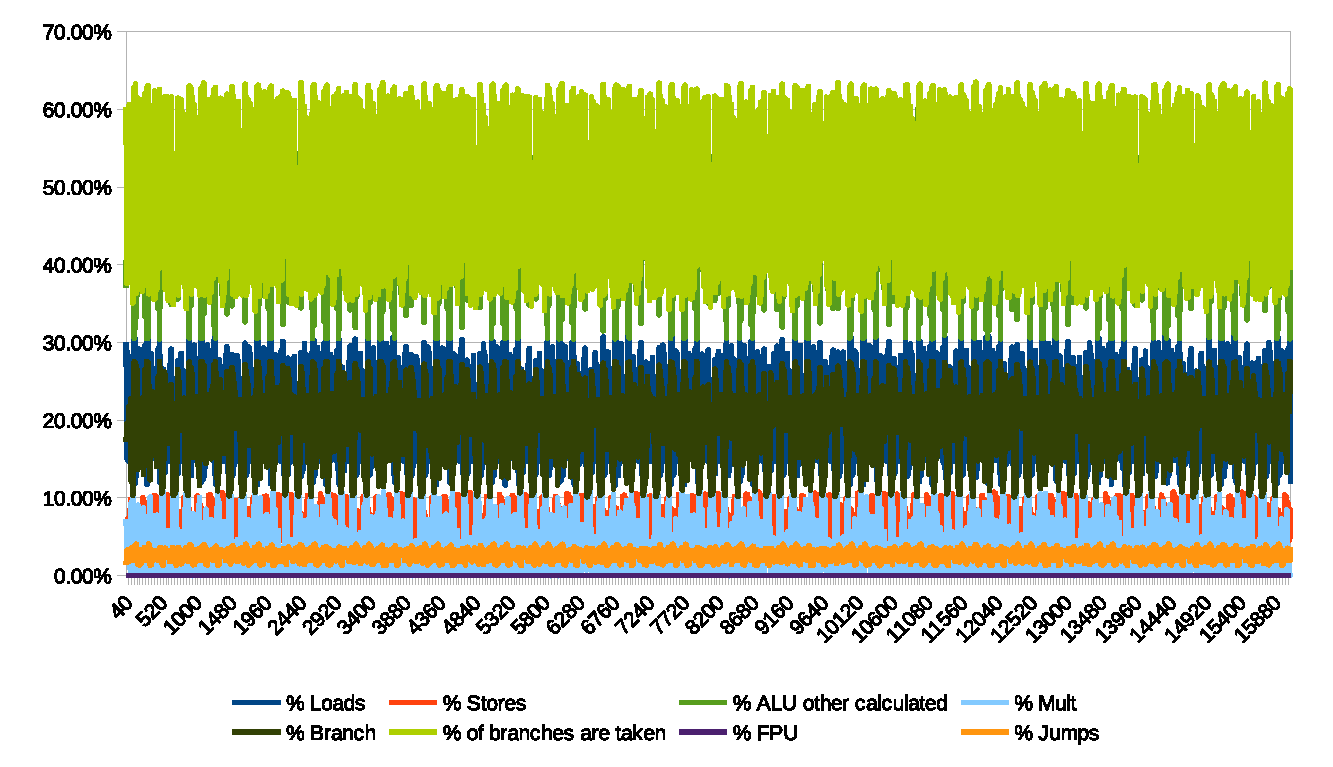
\includegraphics[height=0.26\textheight]{img/graph/coremark/coremark_inst.eps}
        \caption{Instruction behavior over time (ms)}
        \label{fig:res/coremark/inst}
    \end{subfigure}
    \begin{subfigure}{\textwidth}
        \centering
        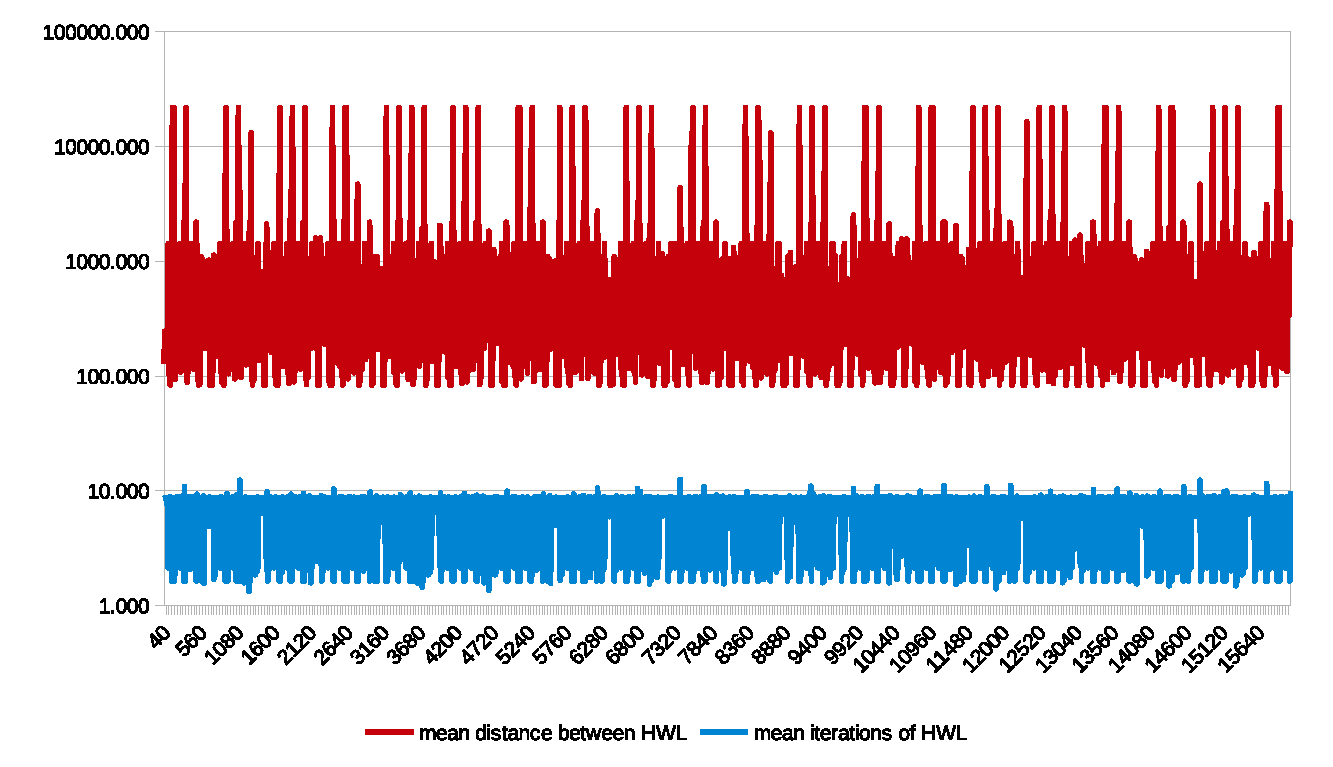
\includegraphics[height=0.26\textheight]{img/graph/coremark/coremark_hwl.eps}
        \caption{\ac{HWL} behavior over time (ms)}
        \label{fig:res/coremark/hwl}
    \end{subfigure}
    \begin{subfigure}{\textwidth}
        \centering
        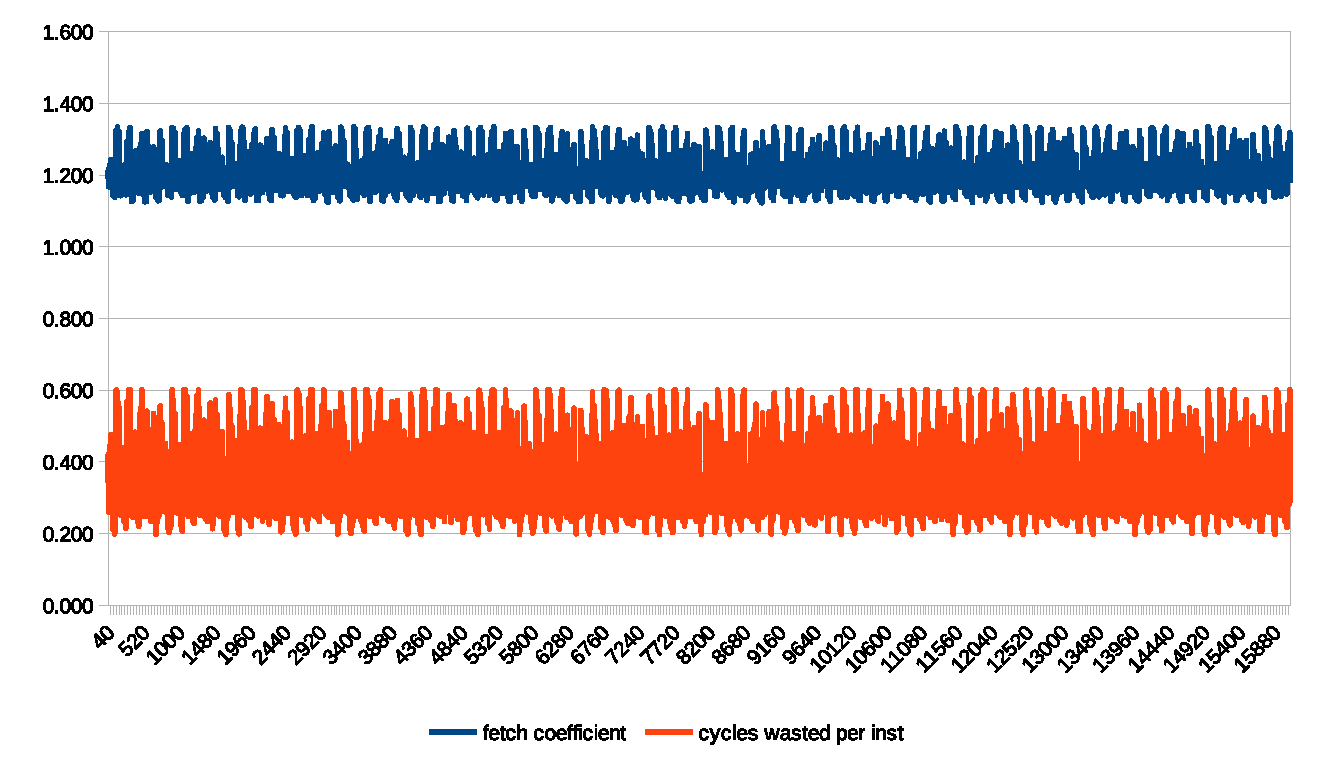
\includegraphics[height=0.26\textheight]{img/graph/coremark/coremark_fetch_waste.eps}
        \caption{Fetch coefficient and cycles wasted per instruction over time (ms)}
        \label{fig:res/coremark/fetch_waste}
    \end{subfigure}
    \caption{Performance over time: Coremark}
    \label{fig:res/coremark}
\end{figure}

% sglib-combined   
\begin{figure}
    \begin{subfigure}{\textwidth}
        \centering
        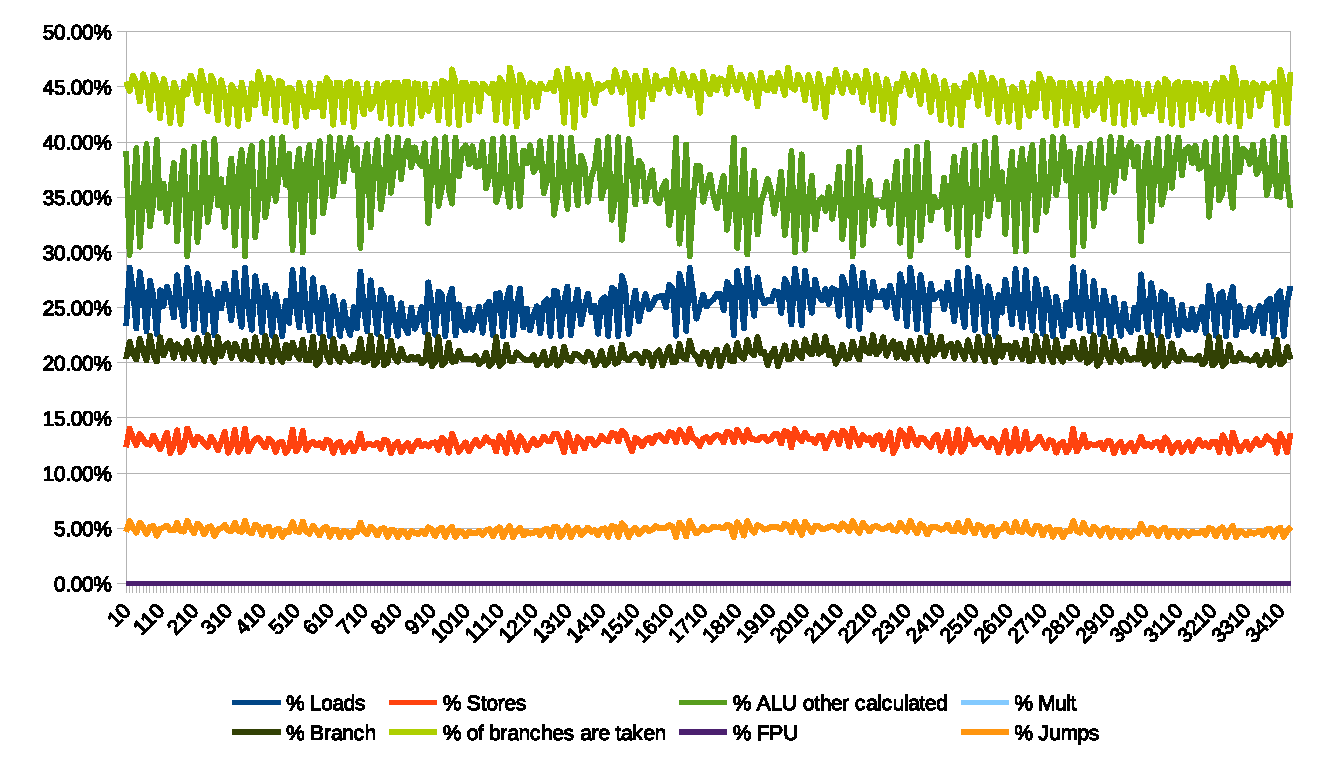
\includegraphics[height=0.26\textheight]{img/graph/embench/sglib-combined_inst.eps}
        \caption{Instruction behavior over time (ms)}
        \label{fig:res/sglib/inst}
    \end{subfigure}
    \begin{subfigure}{\textwidth}
        \centering
        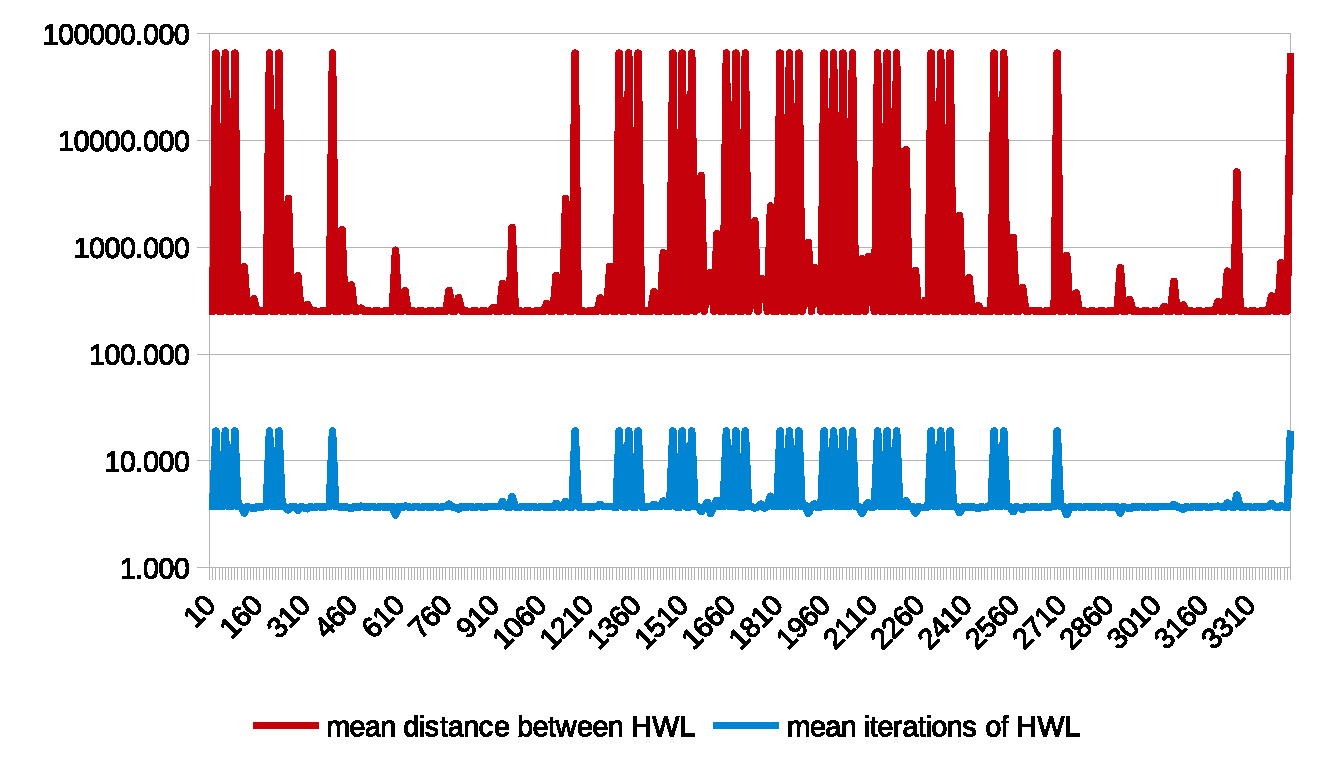
\includegraphics[height=0.26\textheight]{img/graph/embench/sglib-combined_hwl.eps}
        \caption{\ac{HWL} behavior over time (ms)}
        \label{fig:res/sglib/hwl}
    \end{subfigure}
    \begin{subfigure}{\textwidth}
        \centering
        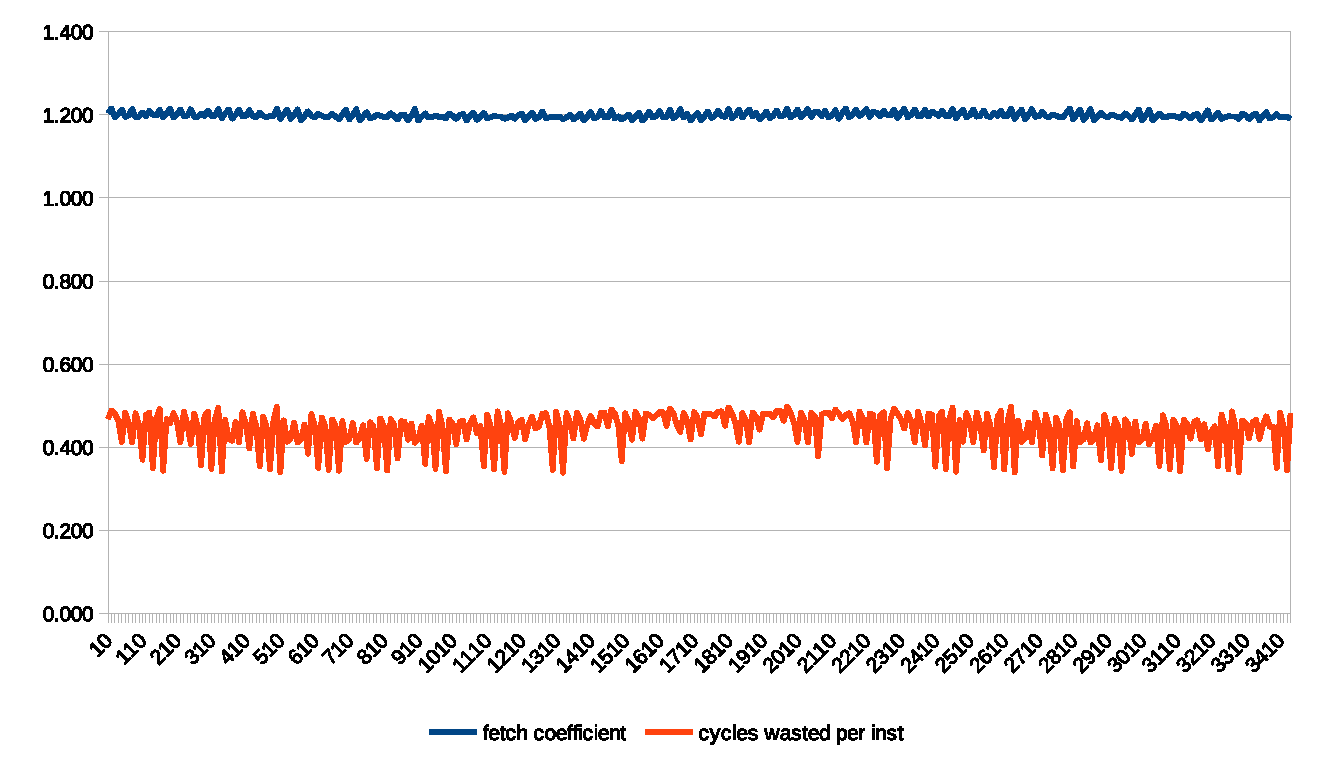
\includegraphics[height=0.26\textheight]{img/graph/embench/sglib-combined_fetch_waste.eps}
        \caption{Fetch coefficient and cycles wasted per instruction over time (ms)}
        \label{fig:res/sglib/fetch_waste}
    \end{subfigure}
    \caption{Performance over time: \texttt{sglib-combined}}
    \label{fig:res/sglib}
\end{figure}

A complete categorization list can be found in table \ref{tab:res/temp/categorization}. So far we do not know if this change of behavior over time influences similarity at all and further study would be required to prove or disprove the necessity of in-flight data. It is additionally important to note that the boundary between group 1 and 3 is rather arbitrary and inherently connected to \texttt{NLYNX\_SECTION\_SIZE} defined in Chapter \ref{ch:arch}. This parameter acts as a smoothing exposure window, as all behavioral changes within its borders are inherently ignored. Expanding the exposure window will inevitably push workloads from group 3 into group 1, whereas shrinking the window will potentially cause the opposite effect.

\begin{table}
    \centering
    \caption{Group categorization of tested workloads}
    \label{tab:res/temp/categorization}
    \begin{tabular}{lll}
        Group 1             & Group 2           & Group 3       \\
        \hline
        embench aha-mont-64 & mibench basicmath & mibench dijkstra    \\
        embench crc32       & mibench bitcount  & embench cubic   \\
        embench edn         & mibench susan     & embench huffbench   \\
        embench minver      & mibench fft       & embench matmult-int \\
        embench nsichneu    &                   & embench nbody   \\
        embench statemate   &                   & embench nettle-aes  \\
        embench ud          &                   & embench nettle-sha256   \\
        Dhrystone           &                   & embench picojpeg    \\
                            &                   & embench qrduino \\
                            &                   & embench sglib-combined  \\
                            &                   & embench slre    \\
                            &                   & embench st  \\
                            &                   & embench wikisort    \\
                            &                   & Coremark    
    \end{tabular}
\end{table}

\section{Metric correlation}
    \label{sec:res/corr}
We calculated the Pearson's correlation coefficient of the different metrics collected, in order to gauge metric interdependence. A coefficient closer to 0 indicates lower correlation, which is desired. A metric is intended to represent a single subsystem in the core and each subsystem is meant to be represented by a single metric. More correlation means more bias towards one particular subsystem in the data. For this calculation, we excluded benchmarks \texttt{factorial}, \texttt{nqueens}, \texttt{tak}, and \texttt{uart\_test} due to their very short length. Table \ref{tab:res/corr/coeff} shows the correlation coefficient between metrics. We see moderate correlation with the mean being about 0.25. 

There are outliers however. We see very strong correlation between the fetch coefficient and the cycles wasted. This is to be expected, as more fetches require more accesses to higher level memory systems which results in more wasted cycles. We also found strong correlation between the share of branch instructions and the fetch coefficient. While this isn't surprising given most workloads seem to favor \emph{branches taken} (as suppose to \emph{branches not taken} implemented by RI5CY), more branches directly translates into more instructions fetched. What was surprising was the rather small correlation between the fetch coefficient and the share of taken branches.

Finally, there appeared to be strong correlation between \ac{HWL} initialization distance and mean \ac{HWL} iteration count (correlation coefficient of $1.0$). This would mean workloads which use \acp{HWL} more often seem to strongly prefer less iterations, while workloads with more distance between \acp{HWL} favor more iterations. This is a misleading conclusion however, as this effect is solely caused by \texttt{embench crc32}, a workload already mentioned for its extensive use of \acp{HWL} in Section \ref{sec:res/control}. Removing this data point from the set drops the correlation coefficient to $0.06$. As mentioned in Section \ref{sec:res/control}, \texttt{embench crc32} likely presents an extreme edge case, where high iteration counts of \acp{HWL} inflate the mean distance between \ac{HWL} initializations.

\begin{table}
    \centering
    \caption{Pearson's correlation coefficient between metrics}
    \resizebox{\textwidth}{!}{%
    \begin{tabular}{l|SSSSSSSSS}
                        & \% Branch     & {\% br. taken}    & \% FPU    & \% Jumps  & {mean dist.}  & {mean it.}    & {fetch coeff.}    & {cycles wasted /} \\
                        &               &                   &           &           & HWL           & HWL           &                   & instruction       \\
        \hline
        \% Mult         & -0.37         &  0.24             & -0.09     & -0.27     &  0.26         &  0.26         & -0.04             & -0.19             \\ \hline
        \% Branch       &               & -0.12             &  0.02     &  0.39     & -0.10         & -0.11         &  0.79             &  0.72             \\ \hline
        \% br. taken    &               &                   & -0.10     & -0.20     &  0.36         &  0.36         & -0.11             & -0.03             \\ \hline
        \% FPU          &               &                   &           & -0.01     & -0.03         & -0.03         & -0.05             &  0.13             \\ \hline
        \% Jumps        &               &                   &           &           & -0.19         & -0.18         &  0.37             &  0.45             \\ \hline
        mean dist. HWL  &               &                   &           &           &               &  0.06         & -0.19             & -0.17             \\ \hline
        mean it. HWL    &               &                   &           &           &               &               & -0.20             & -0.18             \\ \hline
        fetch coeff.    &               &                   &           &           &               &               &                   &  0.82             \\
    \end{tabular}}
    \label{tab:res/corr/coeff}
\end{table}

% Render bibliograhy and acronyms if rendered standalone
\isstandalone
\bibliographystyle{IEEEtran}
\bibliography{bibliography}
\subfile{abbreviations.tex}
\fi

\end{document} 
